\label{sec:ana}
In order to better understand how mutation in a node element impacts CGP, we analyzed the frequency with which the mutation in each element increases the quality of the current solution throughout the evolutionary process. The study was done on the problems labeled small in \cite{benchmark}, using SAM mutation, with 25 independent runs per problem. Each occurrence of improvement was grouped by an arbitrarily chosen interval that represents 4-percentile of the budget and the data is show in plots in \rever[Trocar pelas figuras mais novas]{Figures \ref{fig:2}, \ref{fig:3} and \ref{fig:4}.}
%
\begin{figure}
\centering
  \begin{subfigure}[t]{0.8\textwidth}
    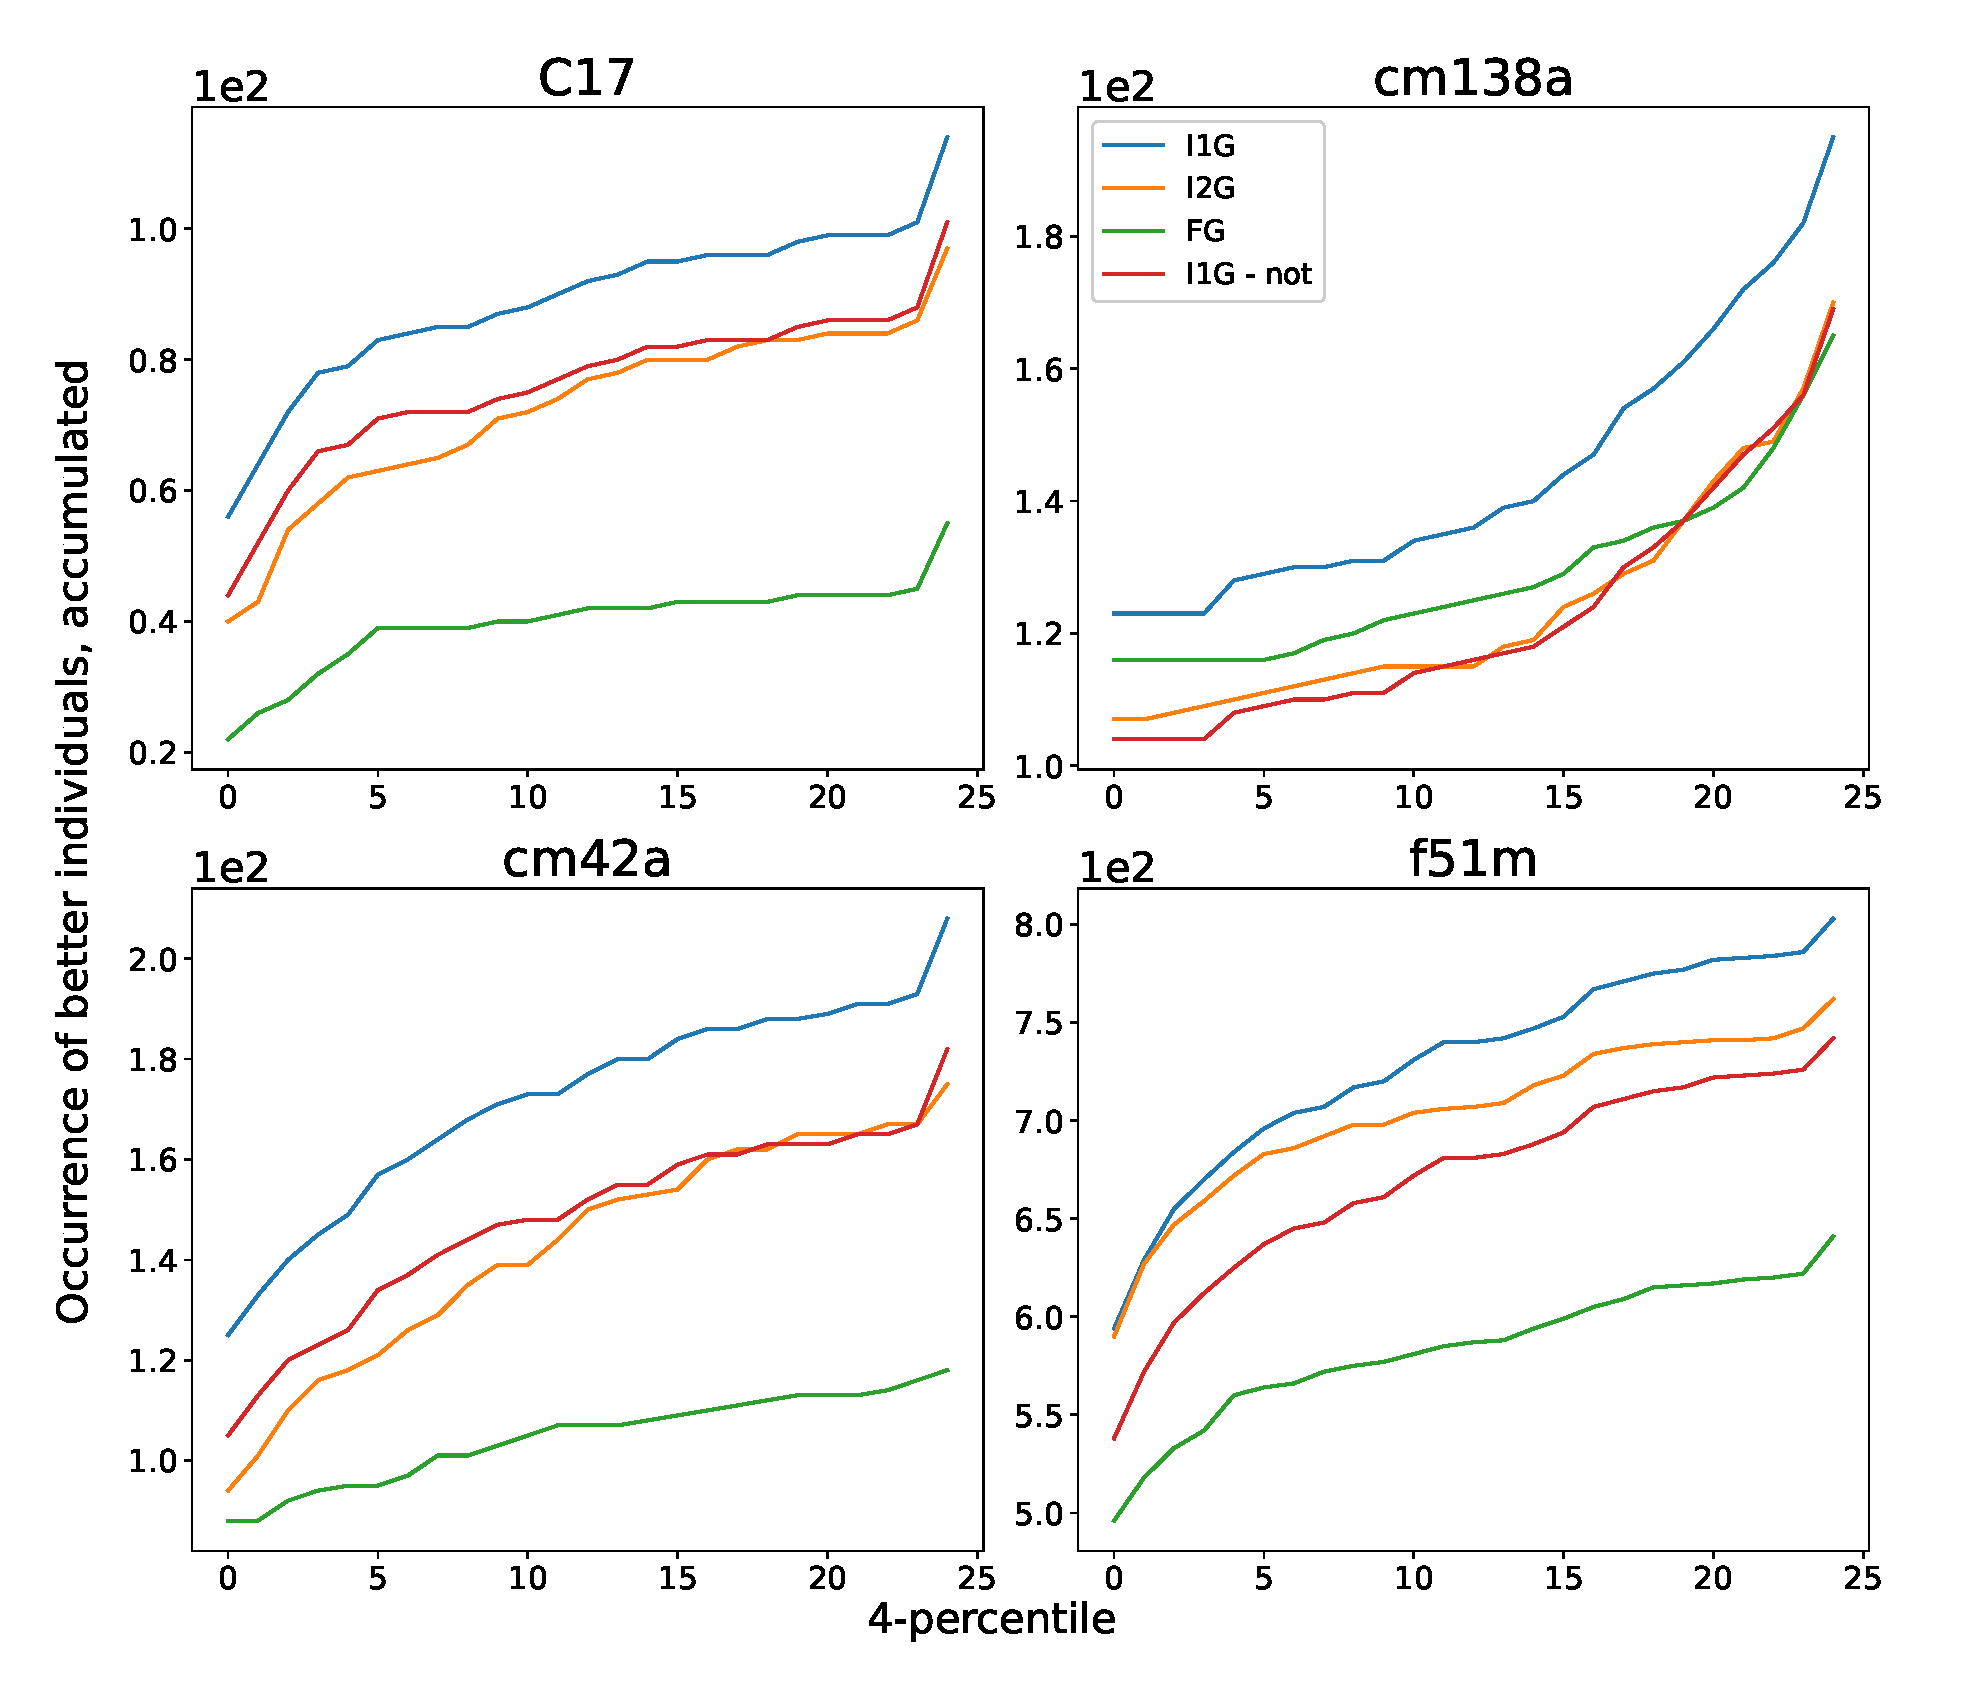
\includegraphics[width=\linewidth]{anal_mut_des_1b.eps}
    \caption{Design phase of the first 4 small problems in the benchmark.} \label{fig:2a}
  \end{subfigure}%
  %\hspace*{\fill}   % maximize separation between the subfigures
  \par
  \begin{subfigure}[c]{0.8\textwidth}
    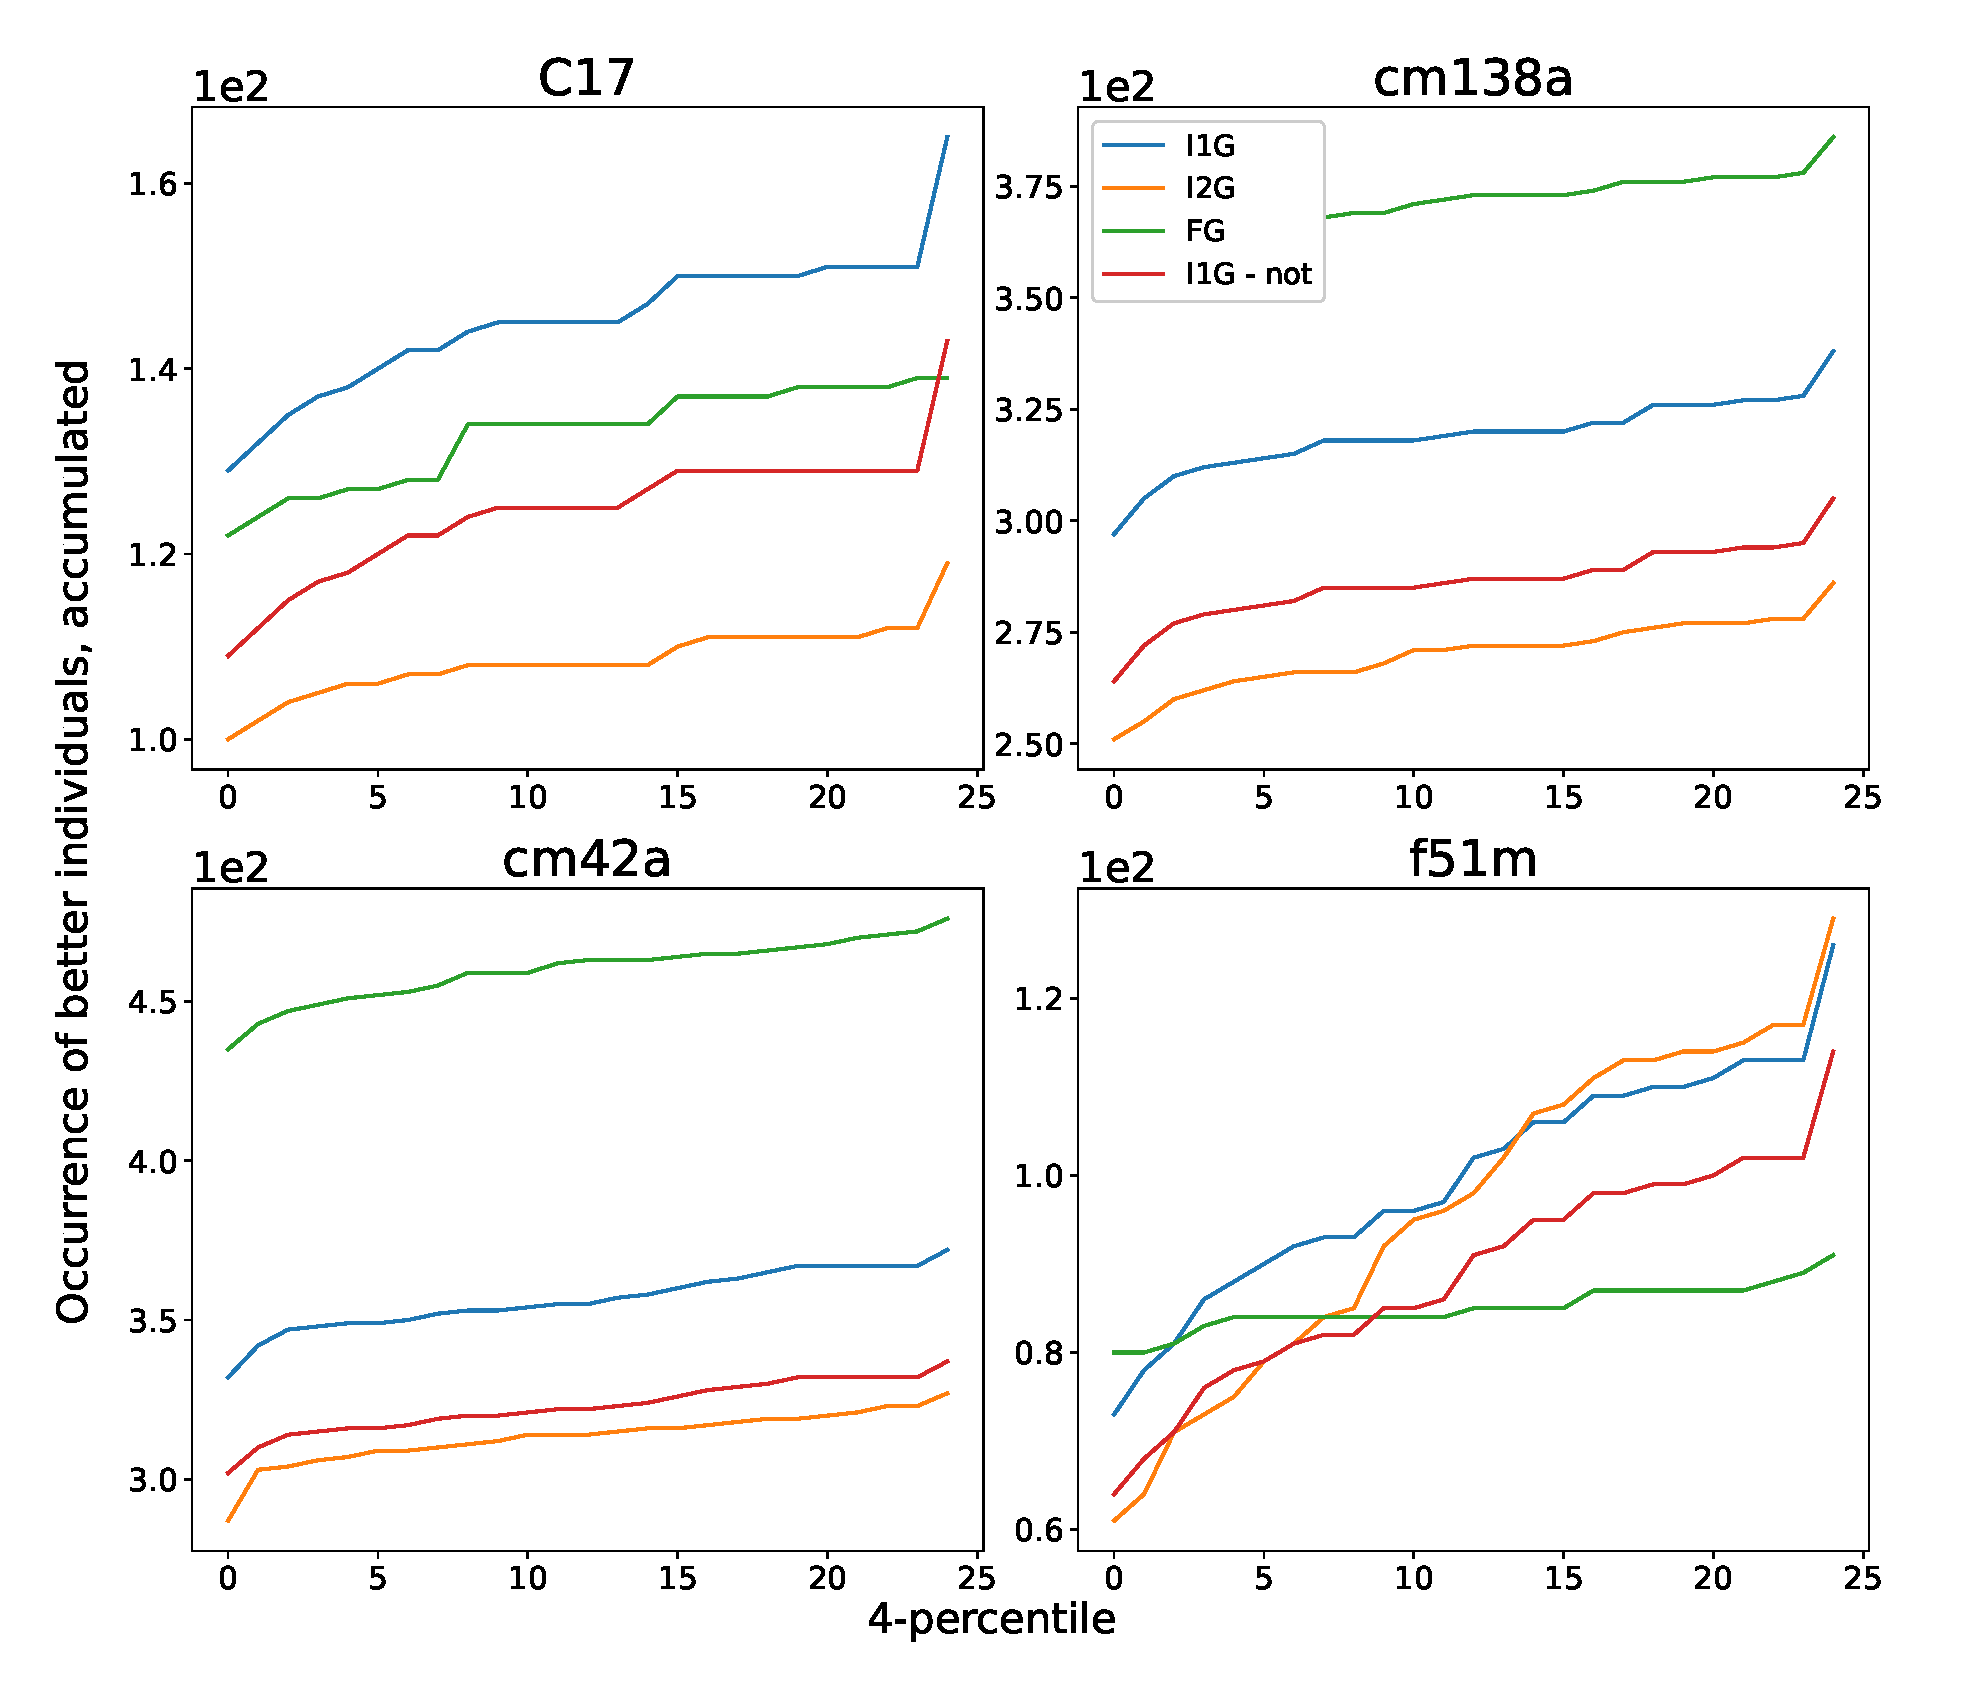
\includegraphics[width=\linewidth]{anal_mut_opt_1b.eps}
    \caption{Optimization phase of the first 4 small problems in the benchmark.} \label{fig:2b}
  \end{subfigure}%
\caption{Comparison between the types of mutation that generate more fit individuals, in the design and optimization phases of the first 4 small problems of the benchmark used in this work. Input address mutations are labeled I1G and I2G and logical gate type mutations as FG} \label{fig:2}
\end{figure}

\begin{figure}
\centering
  \begin{subfigure}[t]{0.8\textwidth}
    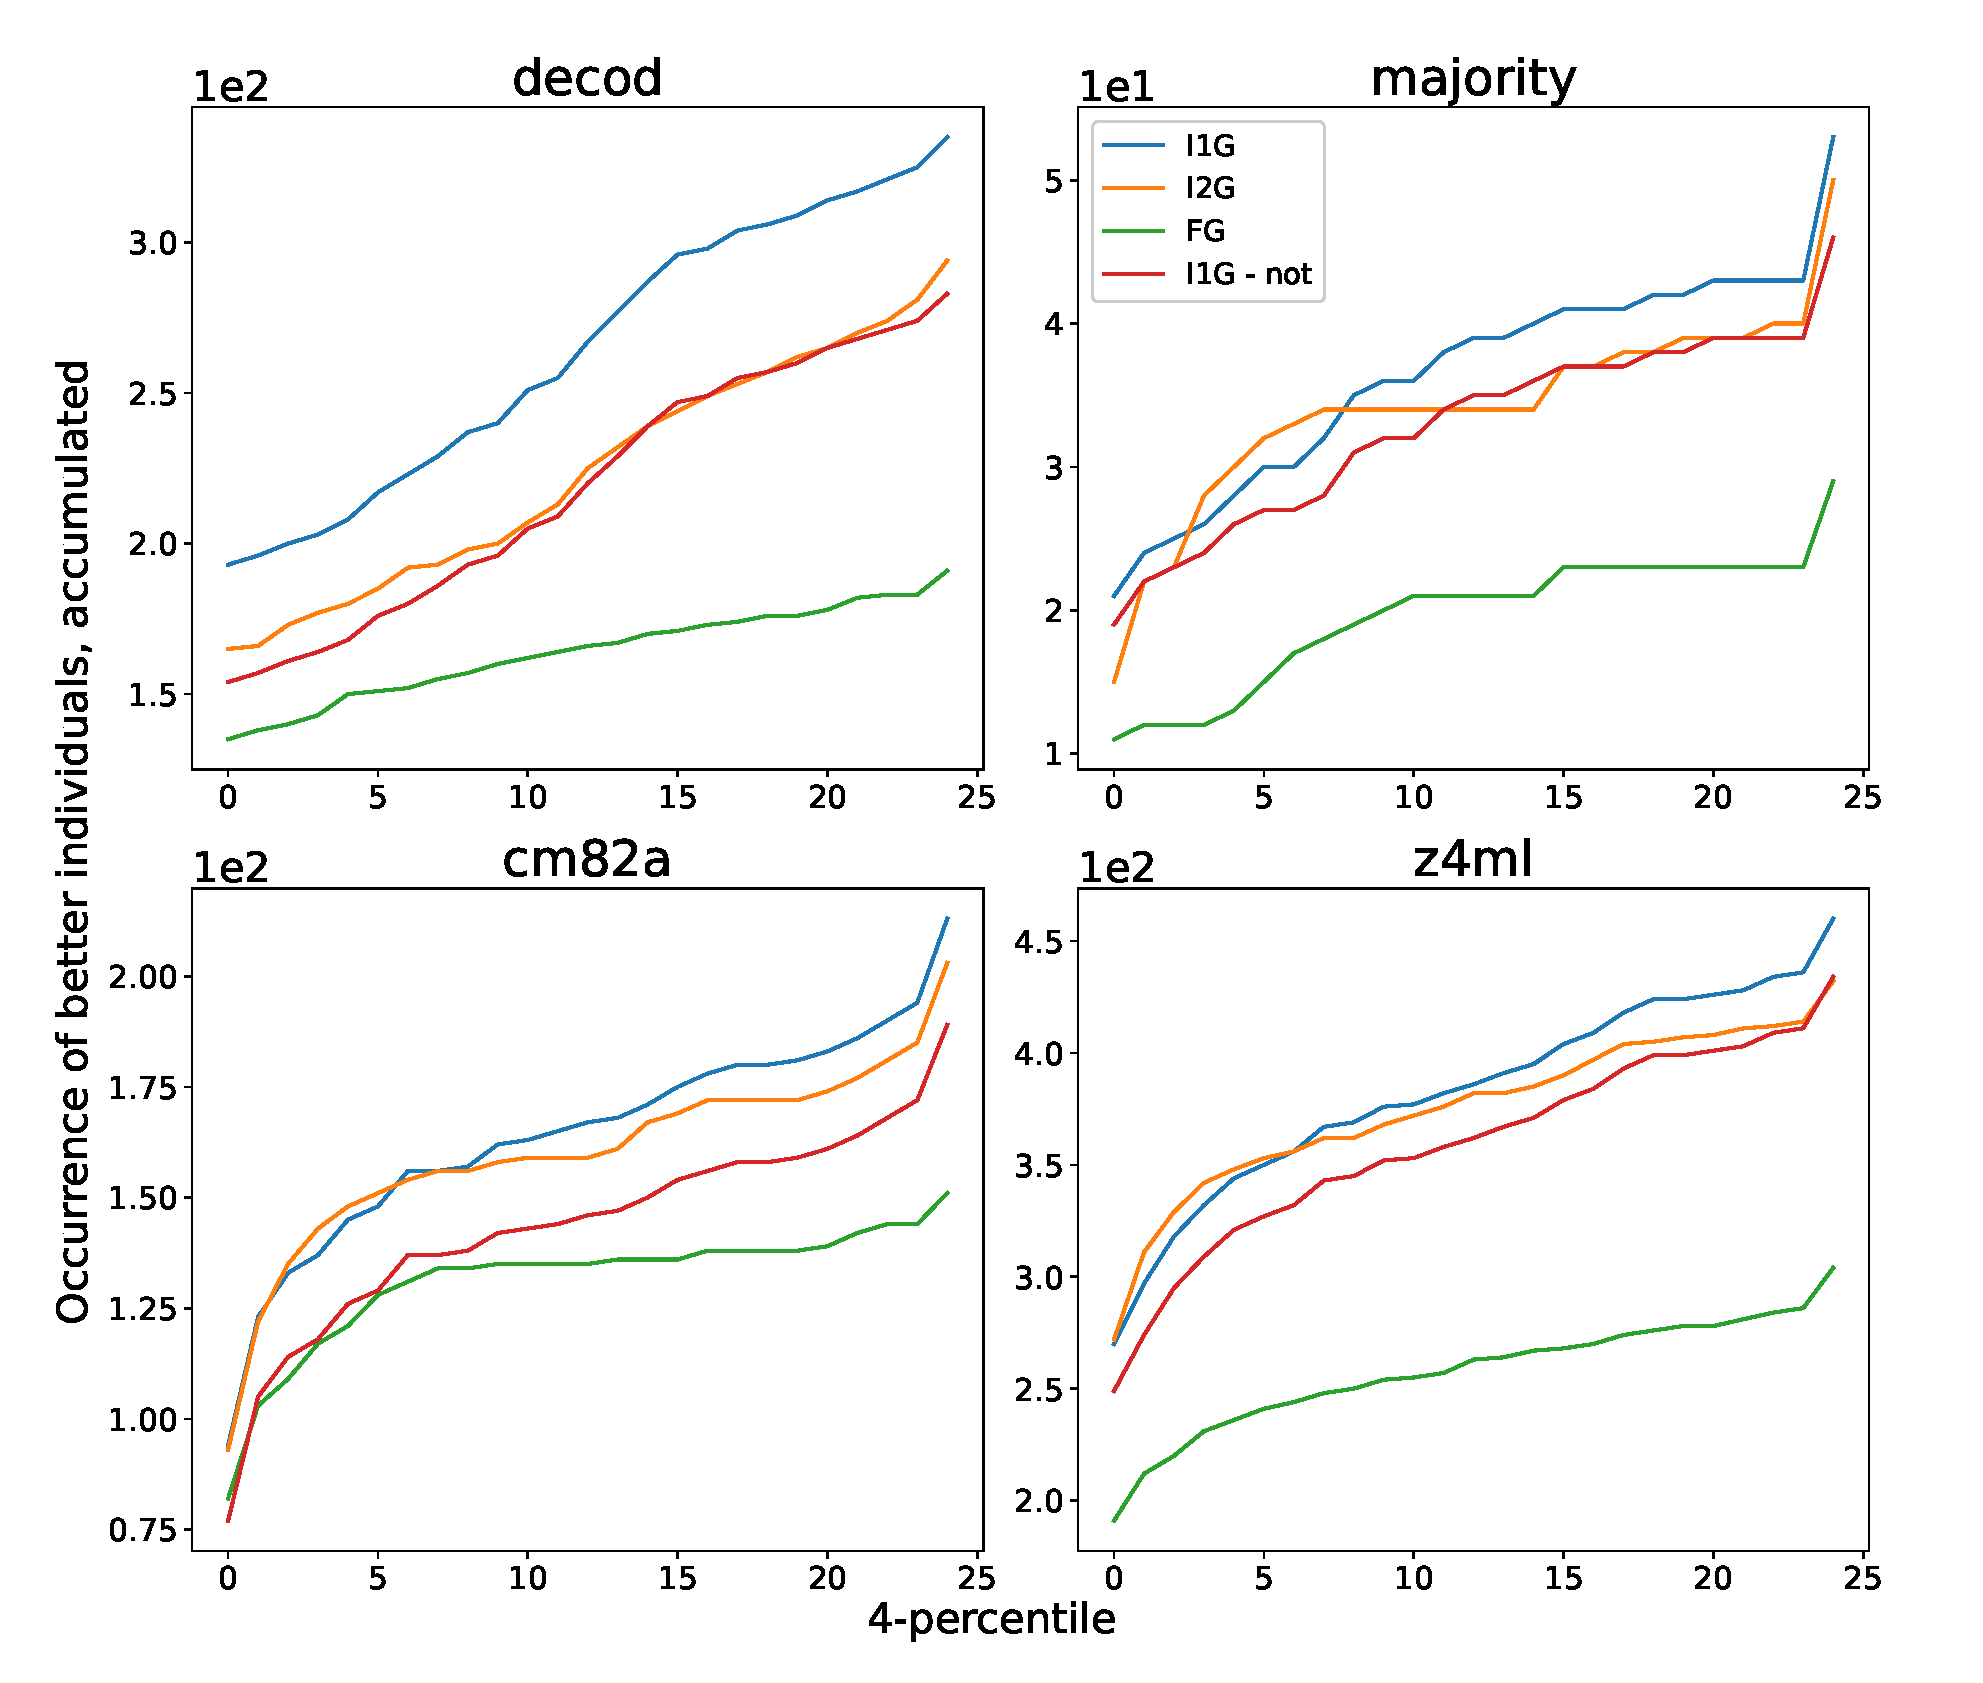
\includegraphics[width=\linewidth]{anal_mut_des_2b.eps}
    \caption{Design phase of the last 4 small problems in the benchmark.} \label{fig:3a}
  \end{subfigure}%
  %\hspace*{\fill}   % maximize separation between the subfigures
  \par
  \begin{subfigure}[c]{0.8\textwidth}
    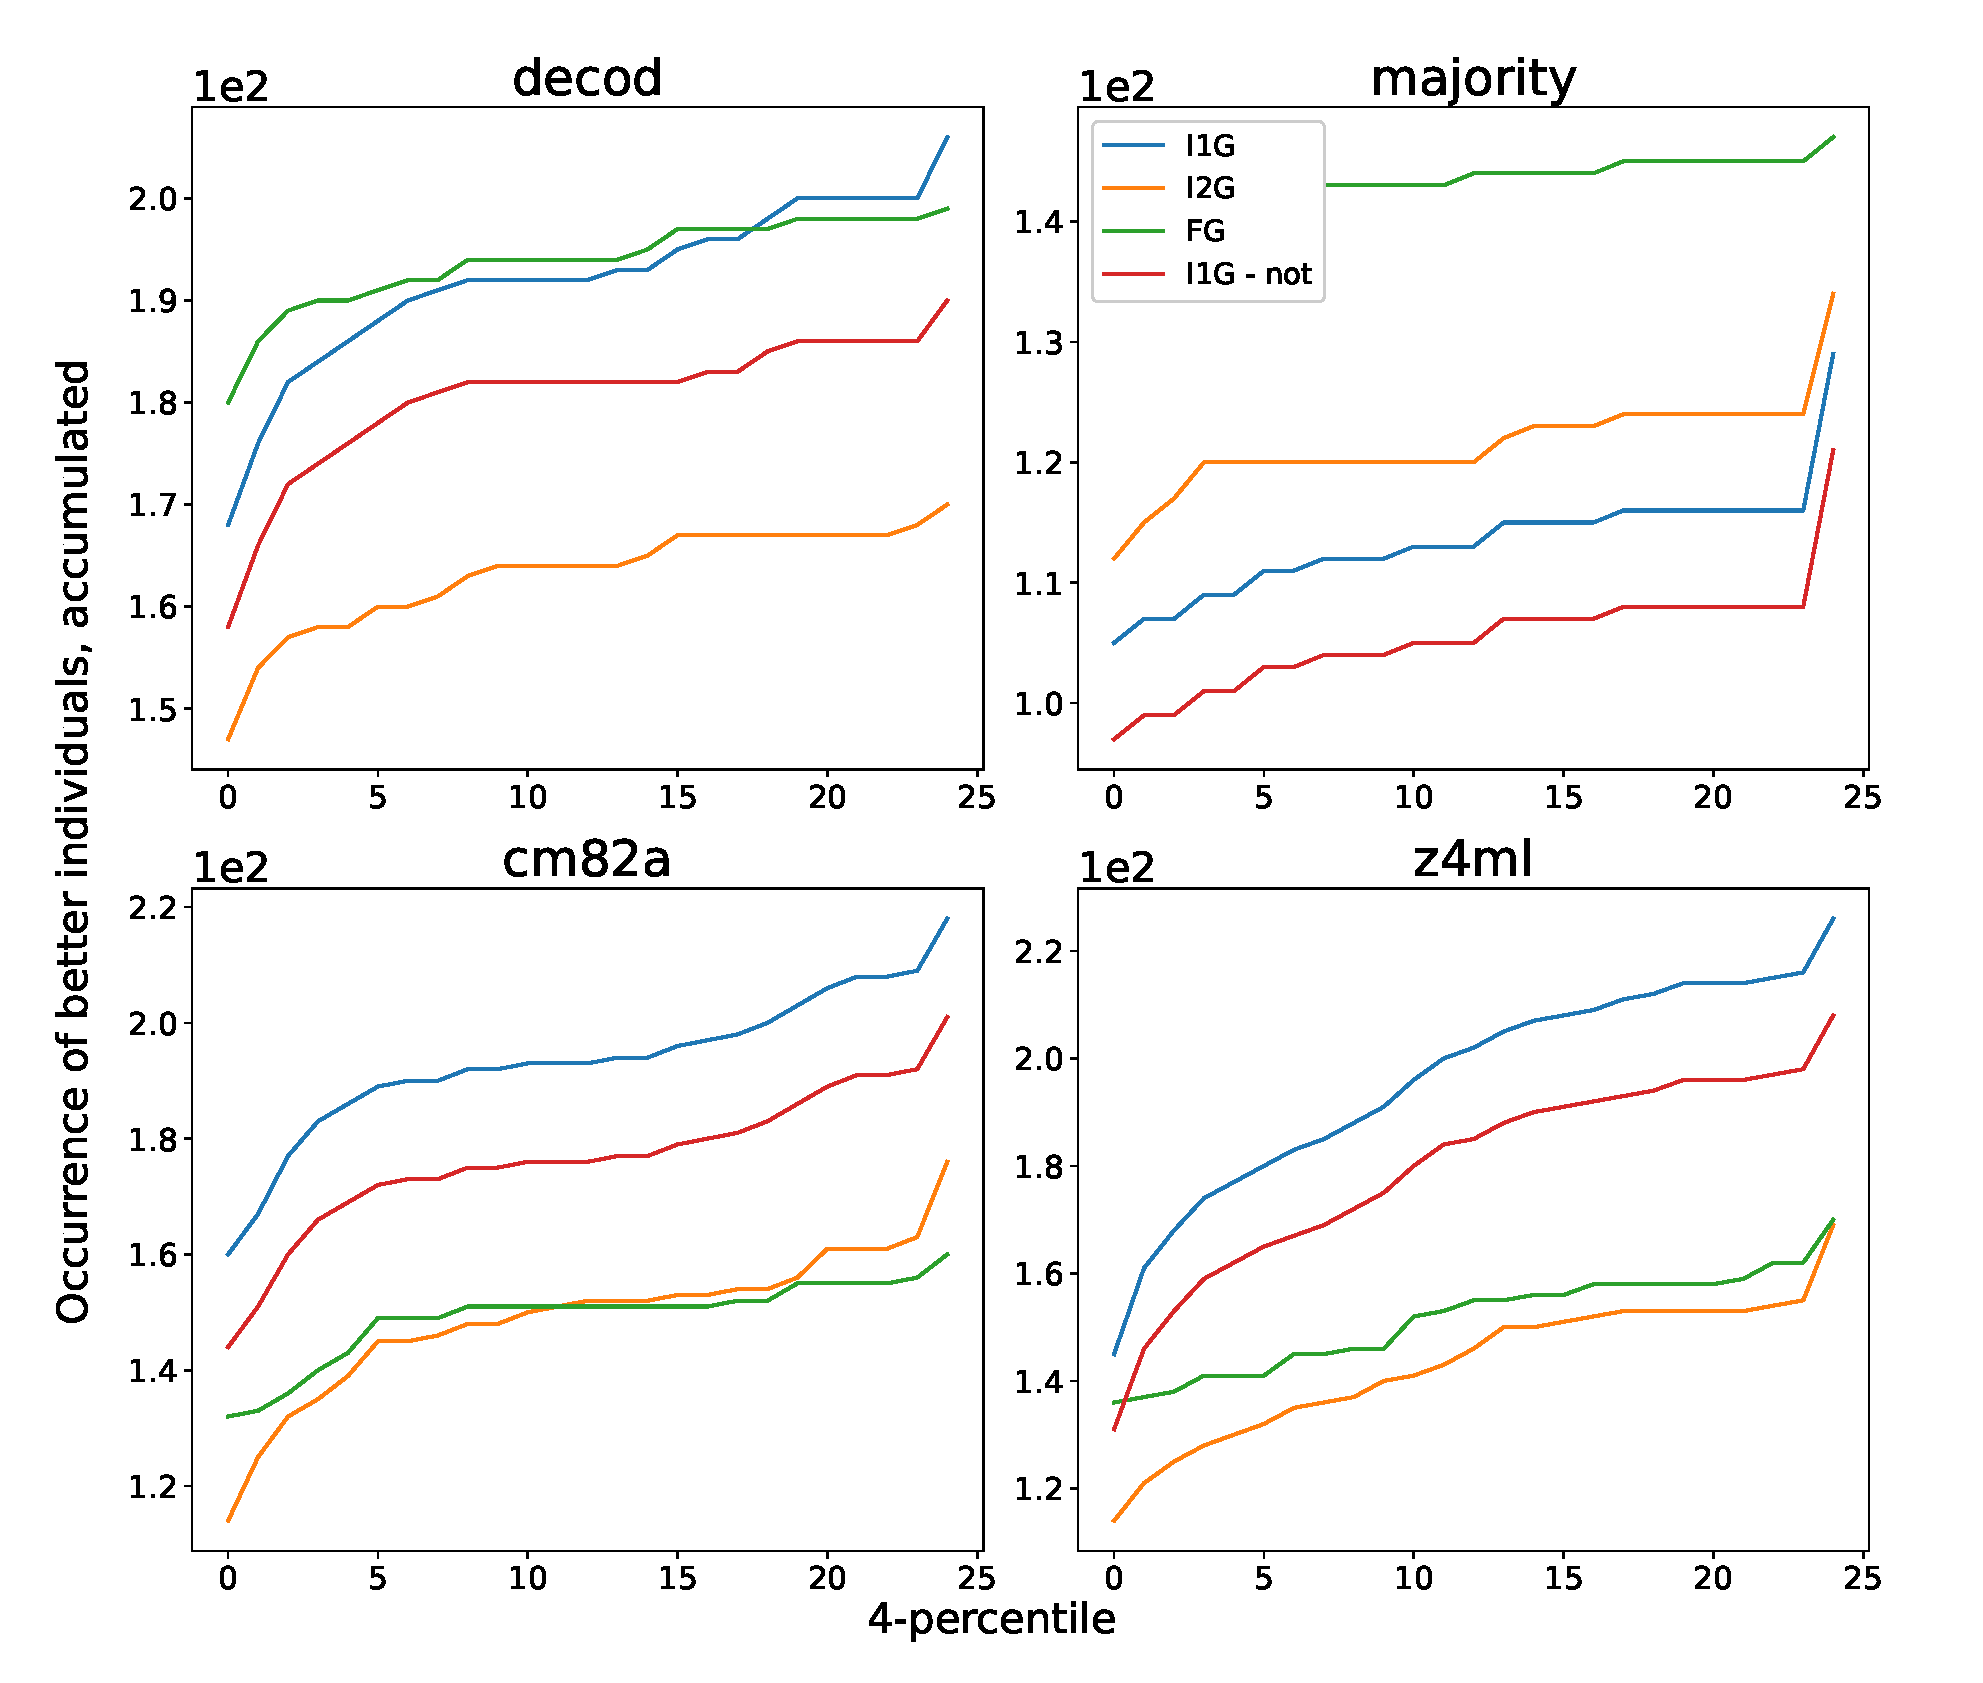
\includegraphics[width=\linewidth]{anal_mut_opt_2b.eps}
    \caption{Optimization phase of the last 4 small problems in the benchmark.} \label{fig:3b}
  \end{subfigure}%
\caption{Comparison between the types of mutation that generate more fit individuals, in the design and optimization phases of the first 4 small problems of the benchmark used in this work. Input address mutations are labeled I1G and I2G and logical gate type mutations as FG} \label{fig:3}
\end{figure}

Figures \ref{fig:2} and \ref{fig:3} represent the cumulative value along the generations of each occurrence of improvement  in the current solution generated by mutations in the 1st input (I1G, Blue), second input (I2G, Orange) and  in the gate type (FG, in green). These values were obtained by the average of the 25 independent runs. One can notice that all problems showed similar patterns for the design phase, with mutations in the first input being responsible for generating better individuals more frequently than mutations in the second input and both (first and second inputs) showing a significantly larger frequency of improvement than mutations in the gate type.

In general, the curves show that mutations in the gate type are less able to generate improvements, having about 50\% to 70\% of the performance of the mutations in the first input, as can be seen by the end values of Figures \ref{fig:2} and \ref{fig:3}. Mutations in the second input performs close to mutations on the first input. However, some differences in the way the curve evolves and the very proportions of the {\tt cm138a} problem already suggest that an adaptive mutation operator is more appropriate than a static bias, and it is expected that such an operator be able to improve CGP's CLC optimization performance. %vou ter que discutir melhor esse paragrafo depois

In the optimization phase, each problem shows a particular pattern. The differences between the frequency of improvement for each type of mutation are less evident. However they are still distinct  to point out that certain mutation policies can be more successful than the others and, thus, a biased operator can take positive advantage of this feature.

For problems where CGP has the highest success rate, most of the objective function and constraints evaluations are used during the optimization phase. This is the case for all the small problems of \cite{benchmark}. However, Figures \ref{fig:2} and \ref{fig:3} show that the total number of times that a better individual appears is almost the same for both the design and optimization phases. A greater difficulty in generating better individuals in the optimization phase is expected, as the reduction of the constraint violation is performed in this phase.

In small problems, CGP generated feasible individuals in about half of the generations. For these generations, the average of feasible individuals was 1.2. Both values can be observed in Table \ref{tab:fac} and in the boxplots in Figures \ref{fig:facgen} and  \ref{fig:facpop}. The plots in Figures \ref{fig:4a} and \ref{fig:4b} show that each type of mutation has a different impact on the generation of feasible individuals, with mutations in the type of logical function appearing to have a greater capacity to offer feasible individuals than mutations in the input. 

\begin{table}[tb]
\caption{Average of generations, during the optimization, in which there was at least one feasible individual generated.}
    \label{tab:fac}
    \centering
    \begin{tabular}{lrr}
\toprule
     Problem &  CGP & Node CGP-RL \\
\midrule
  C17 & 54\% & 33\% \\
  cm42a & 52\% & 30\% \\
  cm82a & 58\% & 35\% \\
  cm138a & 53\% & 28\% \\
  decod & 50\% & 28\% \\
  f51m & 54\% & 32\% \\
  majority & 61\% & 36\%\\
  z4ml & 55\% & 31\% \\
\bottomrule
\end{tabular}
    
\end{table}

\begin{figure}
\centering
  \begin{subfigure}[t]{0.8\textwidth}
    \includegraphics[width=\linewidth]{fig1.eps}
    \caption{Design phase of the first 4 small problems in the benchmark.} \label{fig:4a}
  \end{subfigure}%
  %\hspace*{\fill}   % maximize separation between the subfigures
  \par
  \begin{subfigure}[c]{0.8\textwidth}
    \includegraphics[width=\linewidth]{fig2.eps}
    \caption{Optimization phase of the first 4 small problems in the benchmark.} \label{fig:4b}
  \end{subfigure}%
\caption{Average of feasible individuals per generation where at least one feasible individual occurred.} \label{fig:4}
\end{figure}

\todo{o label fig:4b dessas figuras aparece mais de uma vez }

\begin{figure}
\centering
  \begin{subfigure}[t]{0.8\textwidth}
    \includegraphics[width=\linewidth]{bplotavg1.eps}
    \caption{Design phase of the first 4 small problems in the benchmark.} \label{fig:facpop}
  \end{subfigure}%
  %\hspace*{\fill}   % maximize separation between the subfigures
  \par
  \begin{subfigure}[c]{0.8\textwidth}
    \includegraphics[width=\linewidth]{bplotavg2.eps}
    \caption{Average percentage of generations in the optimization phase where there was the occurrence of at least one feasible child.} \label{fig:4b}
  \end{subfigure}%
\caption{Boxplots on the occurrence of feasible offspring during the optimization process.} \label{fig:facgen}
\end{figure}
